\documentclass{article}
\usepackage{amsmath}
\usepackage{booktabs}
\usepackage{color}
\usepackage{graphicx}
\usepackage{listings}
\usepackage{pgfplotstable}
\usepackage{pgfplots}
\usepackage{siunitx}
\usepackage{tikz}
\usepackage{csvsimple}

\lstset{
  language=Perl,
  basicstyle=\small\sffamily,
  numbers=left,
  numberstyle=\tiny,
  frame=tb,
  tabsize=4,
  columns=fixed,
  showstringspaces=false,
  showtabs=false,
  keepspaces,
  commentstyle=\color{red},
  keywordstyle=\color{blue}
}

\pgfplotsset{compat=newest} % place the legend below the plot
\usepgfplotslibrary{units} % display units nicely

\sisetup{round-mode = places, round-precision = 2}

\title{Penetration Test Report}
%\date{}
\author{Mo Khan}

\begin{document}
\pagenumbering{gobble}
\maketitle
\newpage
\tableofcontents
\newpage
\pagenumbering{arabic}

\section{Executive Summary}

Hello World!

\subsection{Summary of Results}

Structuring a document is easy!

\subsubsection{Subsubsection}

More text.

\paragraph{Paragraph}

Some more text.

\subparagraph{Subparagraph}

Even more text.

\newpage
\section{Attack Narrative}
\subsection{Wordpress Exploitation}
\subsection{Wordpress Plugin Unintended File Type Upload}
\subsection{Linux Local Privilege Escalation}
\subsection{Maintaining Access to Compromised Webserver}
\subsection{Vulnerable Splunk Installation}
\subsection{Domain Privilege Escalation}
\subsection{Attacker Control of Archmake Transactions}

\newpage
\section{Recon}
\subsection{Information}
\subsubsection{DNS}

List out entries found in the /etc/hosts file.

\subsubsection{IP Ranges}

Use genlist to generate a list of ip addresses found.

\subsubsection{Domain names}

\csvautotabular{hosts.csv}

\subsection{Diagrams and spreadsheets}
\subsection{Tools}

\newpage
\section{Mapping}
\subsection{Open Ports}
\subsection{Service version}

\csvautotabular{ports.csv}

\noindent The following command :
\begin{lstlisting}[language=bash]
$ nmap -sV localhost

Starting Nmap 7.01 ( https://nmap.org ) at 2016-02-08 12:02 MST
Nmap scan report for localhost (127.0.0.1)
Host is up (0.00036s latency).
Other addresses for localhost (not scanned): ::1
Not shown: 998 closed ports
PORT     STATE SERVICE    VERSION
2222/tcp open  ssh        OpenSSH 5.3 (protocol 2.0)
3000/tcp open  tcpwrapped

Service detection performed. Please report any incorrect results at https://nmap.org/submit/ .
Nmap done: 1 IP address (1 host up) scanned in 8.78 seconds

\end{lstlisting}

\subsection{Exploits Available}

\newpage
\section{Discovery}
\subsection{Vulnerabilities for metasploitable.sait230.ca}
\subsection{Vulnerabilities for tomcat-apache.sait230.ca}
\subsection{Vulnerabilities for bwa.sait230.ca}
\subsection{Vulnerabilities for ultimatelamp.sait230.ca}
\subsection{Tools}

\newpage
\section{Exploitation}
\subsection{Exploits for metasploitable.sait230.ca}
\subsection{Exploits for tomcat-apache.sait230.ca}
\subsection{Exploits for bwa.sait230.ca}
\subsection{Exploits for ultimatelamp.sait230.ca}

\newpage
\section{Conclusion}
\subsection{Recommendations}
\subsection{Risk Rating}

\newpage
\section{Appendix A: Vulnerability Detail and Mitigation}
\subsection{Risk Rating Scale}
\subsection{Unprotected WP-Admin Access}
\subsection{Vulnerable Wordpress Search Plugin}

\begin{equation*}
	f(x) = x^2
\end{equation*}

This is some example text\footnote{\label{myfootnote}Hello footnote}.

\begin{figure}[h!]
	\includegraphics[width=\linewidth]{images/screenshot.png}
	\caption{A boat.}
	\label{fig:boat1}
\end{figure}

Figure~\ref{fig:boat1} shows a boat.

\begin{table}[h!]
	\centering
	\caption{Caption for the table.}
	\label{tab:table1}
	\begin{tabular}{l|c||r}
		1 & 2 & 3\\
		\hline
		a & b & c\\
	\end{tabular}
\end{table}

I'm referring to footnote~\ref{myfootnote}.

\begin{table}[h!]
	\centering
	\caption{Caption for the table.}
	\label{tab:table2}
	\begin{tabular}{ccc}
		\toprule
		Some & actual & content\\
		\midrule
		prettifies & the & content\\
		as & well & as\\
		using & the & booktabs package\\
		\bottomrule
	\end{tabular}
\end{table}

\newpage
\begin{table}
	\caption{Dummy table}
\end{table}

\newpage
\begin{table}[h!]
	\begin{center}
		\caption{Autogenerated table from csv file}
\label{table4}
		\pgfplotstabletypeset[
			multicolumn names, % allows to have multicolumn names
			col sep=comma, % the seperator in our .csv file
			display columns/0/.style={column name=$Value 1$, column type={S},string type},
			display columns/1/.style={column name=$Value 2$, column type={S},string type},
			every head row/.style={before row={\toprule}, after row={\si{\ampere} & \si{\volt}\\ \midrule}},
			every last row/.style={after row=\bottomrule}, % rule at bottom
		]{table.csv} % filename/path to file
	\end{center}
\end{table}

\newpage
\begin{figure}[h!]
  \begin{center}
    \begin{tikzpicture}
      \begin{axis}[
          width=\linewidth,
          grid=major,
          grid style={dashed,gray!30},
          xlabel=X Axis $U$,
          ylabel=Y Axis $I$,
          x unit=\si{\volt},
          y unit=\si{\ampere},
          legend style={at={(0.5,-0.2)},anchor=north},
          x tick label style={rotate=90,anchor=east}
        ]
        \addplot
        % select columns by using actual column names in csv.
        table[x=column 1,y=column 2, col sep=comma] {table.csv};
        \legend{Plot}
      \end{axis}
    \end{tikzpicture}
    \caption{My first autogenerated plot.}
  \end{center}
\end{figure}

\newpage
\begin{figure}[h!]
  \begin{center}
    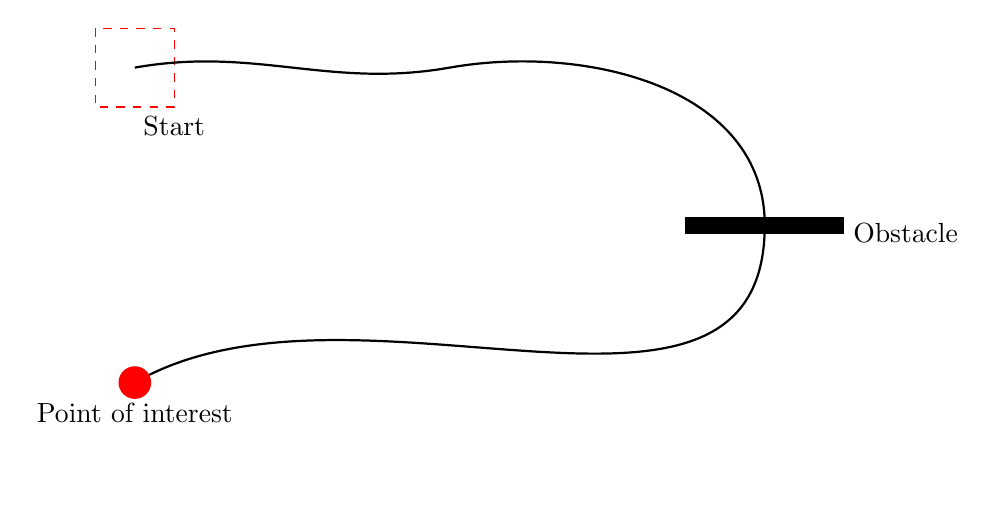
\begin{tikzpicture}
      \draw [red,dashed] (-2.5,2.5) rectangle (-1.5,1.5) node [black,below] {Start};
      \draw [thick] (-2,2)
      to [out=10,in=190] (2,2)
      to [out=10,in=90] (6,0)
      to [out=-90,in=30] (-2,-2);
      \draw [fill] (5,0.1) rectangle (7,-0.1) node [black,right] {Obstacle};
      \draw [red,fill] (-2,-2) circle [radius=0.2] node [black,below=4] {Point of interest}; % draw a circle
    \end{tikzpicture}
    \caption{Example graphic made with tikz.}
  \end{center}
\end{figure}

\newpage
Perl code
\lstinputlisting[language=Perl]{script.pl}

Ruby code
\lstinputlisting[language=Ruby]{script.rb}

Bash script
\lstinputlisting[language=Bash]{script.sh}

\newpage
\begin{appendix}
	\listoffigures
	\listoftables
\end{appendix}

\end{document}
